\documentclass[border=10pt]{standalone}
\usepackage{tikz}
\usetikzlibrary{arrows.meta,calc}

\begin{document}
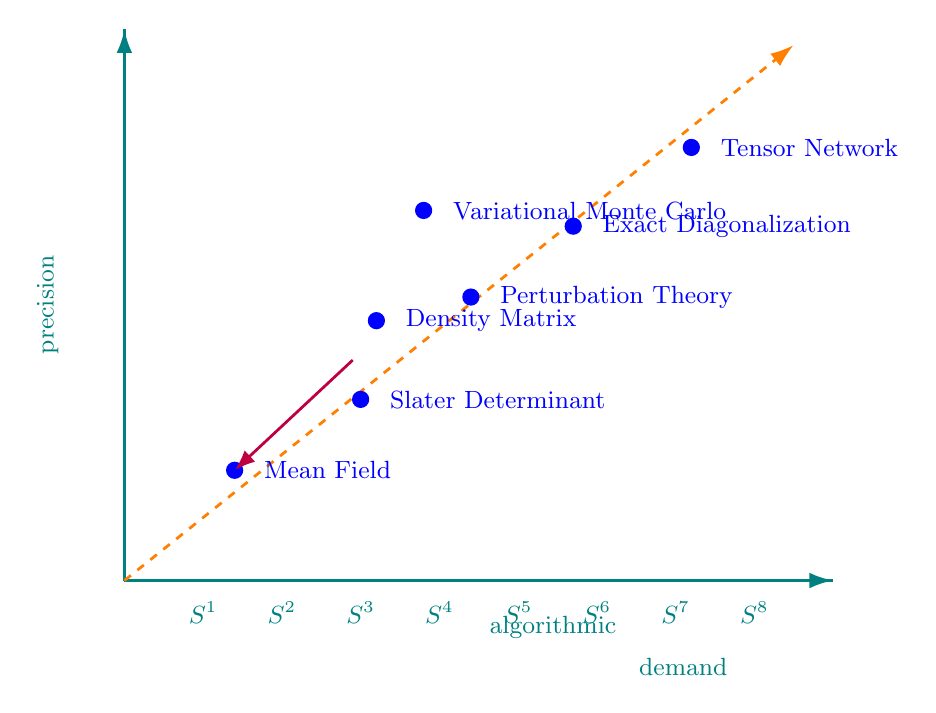
\begin{tikzpicture}[>=Latex,
  axis/.style={line width=1.2pt, teal},
  diagline/.style={line width=1pt, dashed, orange},
  method/.style={circle, fill=blue, inner sep=2.2pt},
  note/.style={blue, font=\small},
  ticklabel/.style={font=\small, teal},
  every node/.style={font=\small}
]

% Axes
\draw[axis] (0,0) -- (0,7.0);  % y-axis
\draw[axis] (0,0) -- (9.0,0);  % x-axis
% Arrowheads
\draw[axis,-{Latex[length=3mm,width=2mm]}] (0,0) -- (0,7.0);
\draw[axis,-{Latex[length=3mm,width=2mm]}] (0,0) -- (9.0,0);

% Axis labels
\node[axis, rotate=90, anchor=south] at (-0.7,3.5) {precision};
\node[axis, anchor=west] at (4.5,-0.6) {algorithmic};
\node[axis, anchor=west] at (6.4,-1.1) {demand};

% x "ticks" as labels S^1 ... S^8 (no actual ticks)
\foreach \i in {1,...,8} {
  \node[ticklabel, anchor=north] at (\i, -0.15) {$S^{\i}$};
}

% Diagonal dashed line with arrow
\draw[diagline,-{Latex[length=3mm,width=2mm]}] (0,0) -- (8.5,6.8);

% Coordinates for methods (estimated)
\coordinate (MeanField) at (1.4,1.4);
\coordinate (Slater) at (3.0,2.3);
\coordinate (Density) at (3.2,3.3);
\coordinate (Perturb) at (4.4,3.6);
\coordinate (VMC) at (3.8,4.7);
\coordinate (Exact) at (5.7,4.5);
\coordinate (Tensor) at (7.2,5.5);

% Points and labels
\node[method] at (MeanField) {};
\node[note, anchor=west] at ($(MeanField)+(0.25,0)$) {Mean Field};

\node[method] at (Slater) {};
\node[note, anchor=west] at ($(Slater)+(0.25,0)$) {Slater Determinant};

\node[method] at (Density) {};
\node[note, anchor=west] at ($(Density)+(0.25,0)$) {Density Matrix};

\node[method] at (Perturb) {};
\node[note, anchor=west] at ($(Perturb)+(0.25,0)$) {Perturbation Theory};

\node[method] at (VMC) {};
\node[note, anchor=west] at ($(VMC)+(0.25,0)$) {Variational Monte Carlo};

\node[method] at (Exact) {};
\node[note, anchor=west] at ($(Exact)+(0.25,0)$) {Exact Diagonalization};

\node[method] at (Tensor) {};
\node[note, anchor=west] at ($(Tensor)+(0.25,0)$) {Tensor Network};

% Purple arrow pointing to Mean Field
\draw[->, line width=1pt, purple] ($(MeanField)+(1.5,1.4)$) -- (MeanField);

\end{tikzpicture}
\end{document}